% ============================================================================
%  The optimal racing line -- minimum-lap-time optimal control
%  Technical report -- B.Sc. Computational Engineering Science (CES), RWTH Aachen
%
%  COMPILE: upload this folder (report.tex + figures/) to Overleaf, "Recompile"
%  (pdfLaTeX). Locally: pdflatex report.tex (run twice).
% ============================================================================
\documentclass[11pt,a4paper]{article}

\usepackage[T1]{fontenc}
\usepackage[utf8]{inputenc}
\usepackage{lmodern}
\usepackage[margin=2.3cm]{geometry}
\usepackage{amsmath,amssymb}
\usepackage{graphicx}
\usepackage{booktabs}
\usepackage{siunitx}
\usepackage{caption}
\usepackage{subcaption}
\usepackage[hidelinks]{hyperref}
\usepackage{xcolor}
\usepackage{enumitem}

\sisetup{detect-all}
\graphicspath{{figures/}}
\captionsetup{font=small,labelfont=bf}
\setlist{nosep,leftmargin=1.4em}

% --- RWTH house colours + banner -------------------------------------------
\definecolor{rwthblue}{HTML}{00549F}
\definecolor{rwthblue25}{HTML}{C7DDF2}
\definecolor{rule}{HTML}{8EBAE5}
\newcommand{\rwthbanner}{%
  \noindent\colorbox{rwthblue}{%
    \parbox{\dimexpr\textwidth-2\fboxsep\relax}{%
      \vspace{2.5pt}%
      {\color{white}\textbf{RWTH AACHEN UNIVERSITY}}\hfill
      {\color{white}\footnotesize Computational Engineering Science}%
      \vspace{2.5pt}}}%
  \vspace{1pt}\par\noindent{\color{rule}\rule{\textwidth}{1.3pt}}%
}

\begin{document}

% ---- title block -----------------------------------------------------------
\rwthbanner
\vspace{0.8em}

{\raggedright
  {\LARGE\bfseries The optimal racing line}\\[0.35em]
  {\large Minimum-lap-time optimal control by direct collocation}\\[0.8em]
  {\normalsize Muhammet Emir Fil}\\[0.15em]
  {\small B.Sc.\ Computational Engineering Science, RWTH Aachen \quad\textbullet\quad Technical report, \today}\par
}
\vspace{0.6em}
\noindent{\color{rule}\rule{\textwidth}{0.6pt}}
\vspace{1.0em}

% ---- AIM -------------------------------------------------------------------
\noindent\colorbox{rwthblue25}{%
  \parbox{\dimexpr\textwidth-2\fboxsep\relax}{%
  \vspace{3pt}\textbf{Aim.} Compute the minimum-lap-time racing line as the solution of an
  optimal-control problem rather than drawing it by hand, and verify the result against
  closed-form optima. The goal is a trajectory-optimisation solver, built from the vehicle model
  up, in which the racing line emerges from the tyre-grip limit and the lap time is checked
  against analytical references. The point mass on a friction circle is a deliberate baseline so
  that every term in the dynamics and every entry in the Jacobian is hand-checkable.\vspace{3pt}}}

\vspace{1.0em}

\begin{abstract}
\noindent
The racing line is not drawn, it is computed. Given a track and a tyre-grip limit, the fastest way
round is the solution of a minimum-lap-time optimal-control problem: find the controls (how to
brake, turn, and accelerate) that minimise the time to traverse a fixed arc length, subject to the
vehicle dynamics and the friction limit. This report formulates that problem, removes its free
final time by switching the independent variable to arc length, transcribes it to a nonlinear
program by direct collocation with hand-derived analytic Jacobians, and solves it. On a 2.4\,km
circuit the optimal line is 8.1\,\% faster than the geometric centreline and rides the grip limit
for nearly the whole lap, and its shape (straight-line braking, late apex, power-down on exit)
emerges without being imposed. The result is verified against closed-form optima; the core is
numpy and scipy.
\end{abstract}

% ---------------------------------------------------------------------------
\section{The problem}
% ---------------------------------------------------------------------------
A lap time is a functional of how the car is driven. Minimising it is a free-final-time
optimal-control problem: the final time is the quantity to minimise, which makes the time horizon
itself an unknown. The standard reformulation removes this difficulty by changing the independent
variable from time $t$ to arc length $s$ along the track centreline. The finish is then a fixed
boundary, $s=L$, and the lap time becomes a definite integral to minimise. This is the central
modelling decision and the reason the problem is tractable. The vehicle model is a baseline by
choice: the single-track (bicycle) model is the natural next layer and would warm-start from this
solution.

% ---------------------------------------------------------------------------
\section{Formulation}
% ---------------------------------------------------------------------------
\paragraph{States and controls.} In the Frenet frame attached to the centreline the car has three
states as functions of $s$: lateral offset $n$, heading relative to the track tangent $\xi$, and
speed $v$. The controls are longitudinal and lateral acceleration $(a_t,a_n)$, limited by the
friction circle
\begin{equation}
  a_t^2 + a_n^2 \le (\mu g)^2 .
  \label{eq:friction}
\end{equation}

\paragraph{Dynamics.} With track curvature $\kappa(s)$ and $D = 1 - n\kappa$, the arc-length
dynamics are
\begin{equation}
  \frac{dn}{ds} = D\tan\xi,\qquad
  \frac{d\xi}{ds} = \frac{D\,a_n}{v^2\cos\xi} - \kappa,\qquad
  \frac{dv}{ds} = \frac{D\,a_t}{v\cos\xi},\qquad
  \underbrace{\frac{dt}{ds} = \frac{D}{v\cos\xi}}_{\text{lap-time integrand}} .
  \label{eq:dyn}
\end{equation}
The objective is the lap time $T = \int_0^L (dt/ds)\,ds$. The track is enforced as a bound
$|n| \le \tfrac12 w(s)$, and the lap is closed by periodic boundary conditions
$\mathbf{x}(0)=\mathbf{x}(L)$, which is what makes the optimiser solve the corners coupled (the
line through one corner depends on the next).

\paragraph{Transcription.} The continuous problem is discretised by trapezoidal direct collocation
on $N$ intervals: states and controls at the nodes are the unknowns $\mathbf{z}$, the
dynamics~\eqref{eq:dyn} become equality defect constraints between adjacent nodes,
\begin{equation}
  \mathbf{x}_{k+1} - \mathbf{x}_k - \tfrac12\,\Delta s_k(\mathbf{f}_k + \mathbf{f}_{k+1}) = \mathbf{0},
  \label{eq:defect}
\end{equation}
and the objective is the trapezoidal sum of $dt/ds$. This yields a nonlinear program (NLP) solved
with scipy's SLSQP. The solver is handed exact analytic Jacobians of the objective gradient, the
defects~\eqref{eq:defect}, and the friction constraint~\eqref{eq:friction}, derived by hand from
Eq.~\eqref{eq:dyn} rather than finite-differenced.

\paragraph{Conditioning.} A closed-circuit NLP is stiff: the states span two orders of magnitude
and the periodic constraint couples the whole lap. Three ingredients make it converge cleanly:
variable scaling to dimensionless decision variables; a quasi-steady-state warm start (the
$g$--$g$-limited speed profile on the centreline, $v=\sqrt{a_\text{max}/|\kappa|}$ with a forward
acceleration pass and a backward braking pass, so the NLP only has to find the line); and mesh
continuation. Together these turned the solve from a failed return into a clean optimum.

% ---------------------------------------------------------------------------
\section{Verification: the solution is correct, not just feasible}
% ---------------------------------------------------------------------------
Tight defects alone only prove the NLP satisfied its own constraints. Correctness is established
against independent references at two levels, the forward model and the optimiser
(Table~\ref{tab:verify}).

\begin{table}[h]
  \centering
  \caption{Verification of the forward car and the optimal-control solver.}
  \label{tab:verify}
  \small
  \begin{tabular}{@{}lll@{}}
    \toprule
    Check & Reference & Result \\
    \midrule
    Analytic Jacobians vs finite difference & exact derivatives        & $< 1.2\times10^{-6}$ \\
    Steady corner radius                    & $v^2 = \mu g R$           & exact \\
    RK4 integration order                   & 4th order                 & slope 4.04 \\
    Skidpad lap time (closed form)          & $T = 2\pi\sqrt{R/\mu g}$  & matches to $-0.2\,\%$ \\
    Mesh convergence of lap time            & trapezoidal $\sim\Delta s^2$ & converges \\
    Friction-circle saturation              & optimal control rides the limit & about 100\,\% at limit \\
    \bottomrule
  \end{tabular}
\end{table}

The two non-trivial checks: the analytic Jacobians match finite differences to better than
$1.2\times10^{-6}$, so the gradients the solver trusts are right; and the converged lap time
matches the closed-form skidpad optimum $T=2\pi\sqrt{R/\mu g}$, a constant-radius lap the model
cannot cheat, to $-0.2\,\%$, with the residual explained by the finite track width. Mesh
refinement confirms the trapezoidal $\mathcal{O}(\Delta s^2)$ convergence.

\begin{figure}[h]
  \centering
  \begin{subfigure}{0.48\textwidth}
    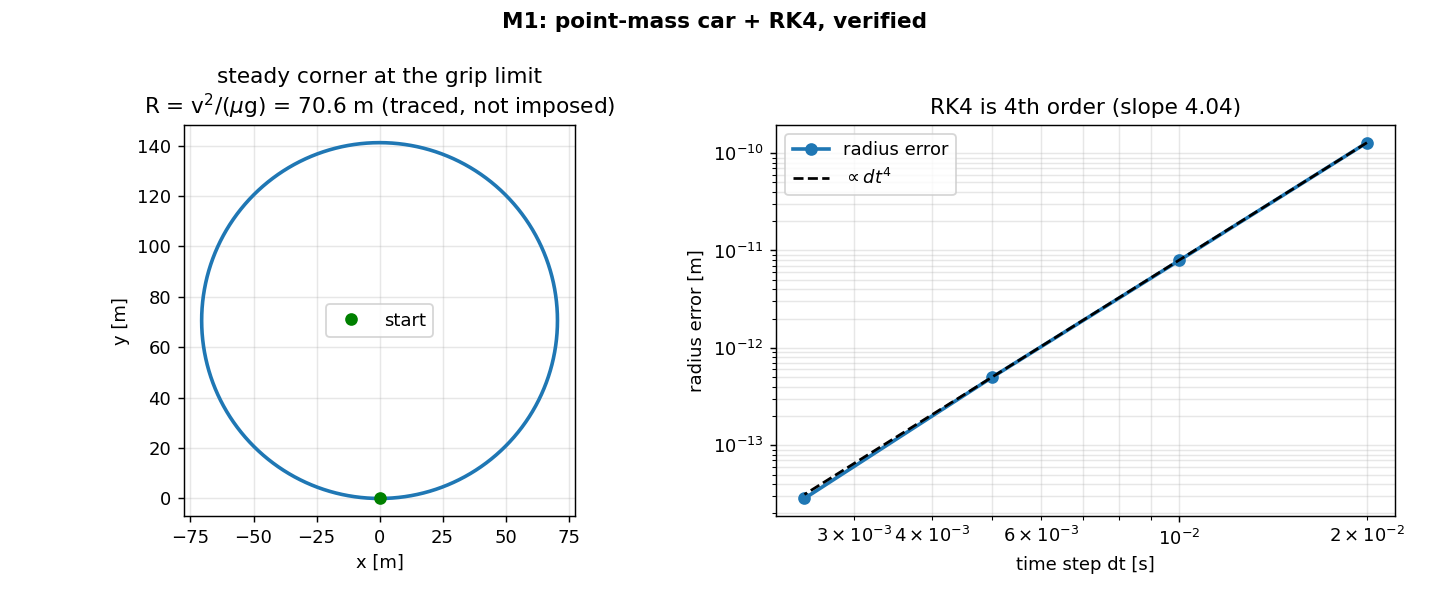
\includegraphics[width=\linewidth]{m1_car_verify.png}
    \caption{Forward car: energy conservation, steady corner $v^2=\mu g R$, RK4 order 4.04.}
  \end{subfigure}\hfill
  \begin{subfigure}{0.48\textwidth}
    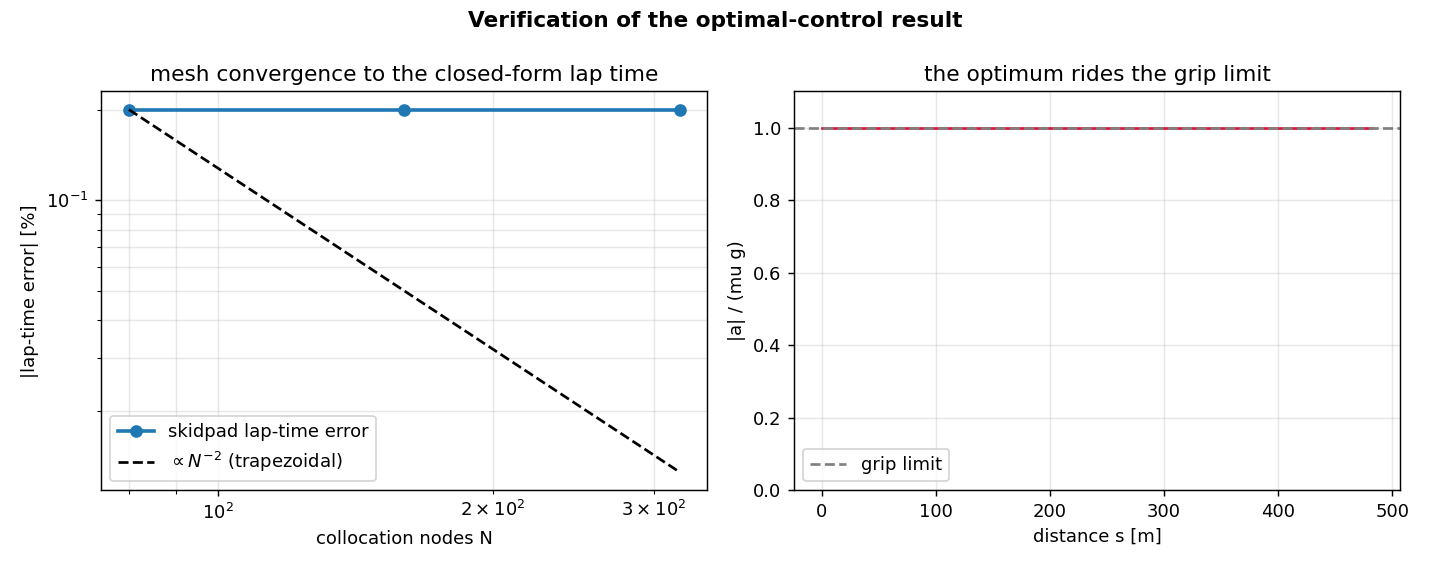
\includegraphics[width=\linewidth]{verify_lap.png}
    \caption{Optimiser: skidpad closed-form match, mesh convergence, friction saturation.}
  \end{subfigure}
  \caption{Verification at both levels: the forward dynamics and the optimal-control solve.}
  \label{fig:verify}
\end{figure}

% ---------------------------------------------------------------------------
\section{Result: the line emerges}
% ---------------------------------------------------------------------------
On a stylised 2.4\,km Grand Circuit ($\mu = 1.5$), the optimal lap is 38.76\,s, against 42.19\,s
for the same car constrained to the geometric centreline. The optimal racing line is therefore
3.43\,s (8.1\,\%) faster, which is the whole value of a racing line. The maximum defect is about
$5\times10^{-11}$: the trajectory satisfies the dynamics to machine precision.

Nothing about the line's shape was imposed. From minimising time under
Eqs.~\eqref{eq:friction}--\eqref{eq:dyn} alone, the solver finds that the fast way round is to
brake in a straight line, use the full track width to straighten the corner (a larger effective
radius buys a higher apex speed), trail-brake to a late apex, and get back to power on exit. The
$g$--$g$ diagram (Fig.~\ref{fig:lap}) shows the car visiting every point on the friction circle and
sitting on it for nearly the whole lap, which is the signature of a time-optimal trajectory.

\begin{figure}[h]
  \centering
  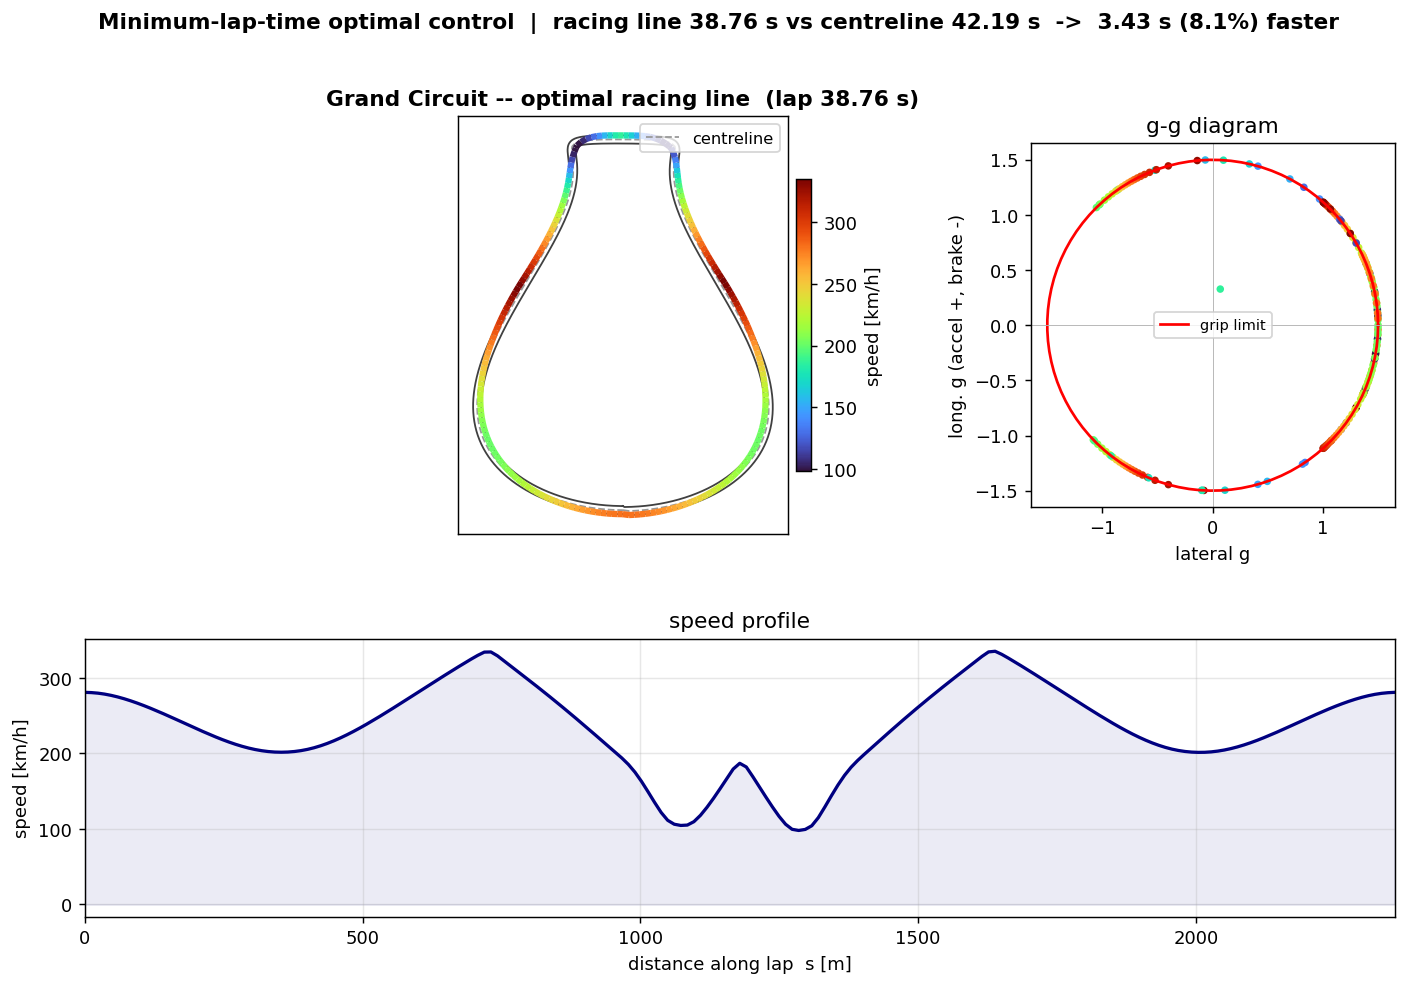
\includegraphics[width=0.95\textwidth]{the_lap.png}
  \caption{The optimal lap. Left: the racing line coloured by speed, straightening the corners
  against the centreline. Middle: the $g$--$g$ diagram saturating the friction circle. Right: the
  speed profile (brake, apex, accelerate). The line is the output of the optimisation, not an
  input.}
  \label{fig:lap}
\end{figure}

% ---------------------------------------------------------------------------
\section{Real car physics on the same core}
% ---------------------------------------------------------------------------
Each real-car effect is one extra term in the dynamics plus its analytic Jacobian row, and all
default off so the baseline stays the pure friction circle: an engine power limit
$a_t \le P/(mv)$, aerodynamic drag $a_\text{drag}=\tfrac12\rho C_d A\,v^2/m$, and downforce, which
makes the grip limit grow with speed,
\begin{equation}
  a_\text{grip}(v) = \mu\big(g + \tfrac12\rho C_l A\,v^2/m\big).
\end{equation}
The $g$--$g$ circle then becomes a speed-dependent performance envelope (Fig.~\ref{fig:aero}): fast
corners pull more $g$ than slow ones (up to $4.7g$ at $310\,\mathrm{km/h}$), which is the defining
feature of a real race car.

% ---------------------------------------------------------------------------
\section{The optimiser as a design tool}
% ---------------------------------------------------------------------------
Because the solve is cheap and warm-starts across parameters, re-solving the lap while sweeping a
parameter turns the model into a trade study (Fig.~\ref{fig:aero}, right): lap time versus grip
(wet to slicks), versus power (diminishing returns), and versus downforce
($40.8\,$s to $27.7\,$s across the swept range). This is what dynamic optimisation is for:
answering ``how much does $+X$ buy'' quantitatively, not drawing a line.

\begin{figure}[h]
  \centering
  \begin{subfigure}{0.48\textwidth}
    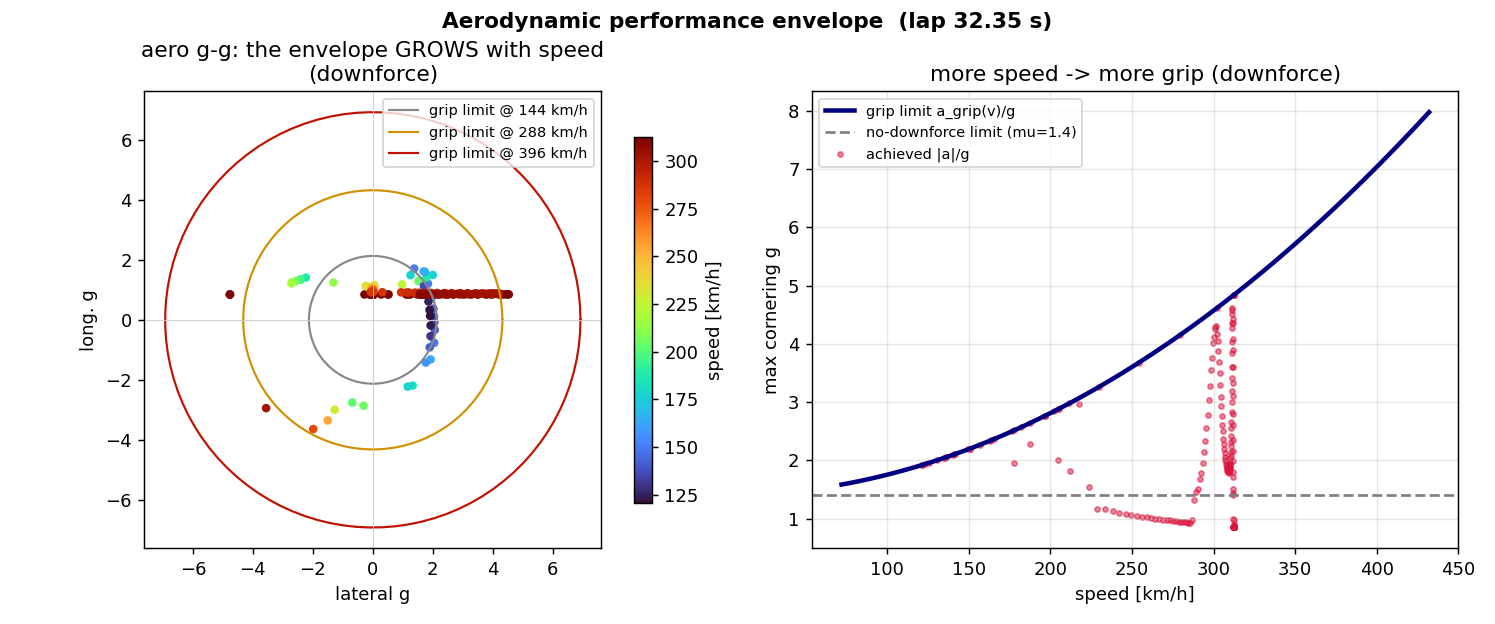
\includegraphics[width=\linewidth]{aero_envelope.png}
    \caption{Speed-dependent $g$--$g$ envelope with downforce.}
  \end{subfigure}\hfill
  \begin{subfigure}{0.48\textwidth}
    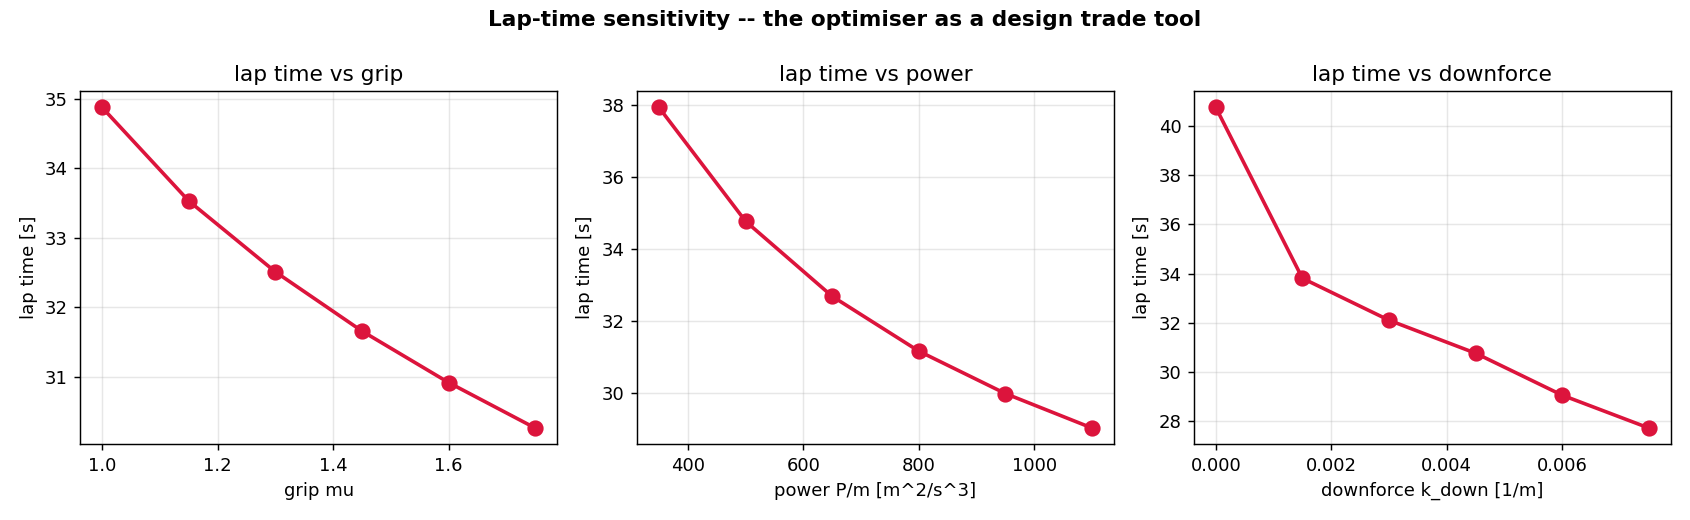
\includegraphics[width=\linewidth]{sensitivity.png}
    \caption{Lap-time sensitivity: grip, power, downforce.}
  \end{subfigure}
  \caption{The same optimal-control core, used for real-car physics and as a design tool.}
  \label{fig:aero}
\end{figure}

% ---------------------------------------------------------------------------
\section{Limitations and outlook}
% ---------------------------------------------------------------------------
\begin{itemize}
  \item The vehicle is a point mass on a friction circle: no load transfer, no yaw dynamics, no
        combined-slip tyre. This is a deliberate, hand-checkable baseline.
  \item The natural next layer is the single-track (bicycle) model with a combined-slip tyre,
        which would warm-start directly from this solution.
  \item SLSQP is a dense SQP and does not scale past $N\!\sim\!250$ nodes; for much finer meshes an
        interior-point solver (IPOPT) exploiting sparsity is the right tool, and the transcription
        and analytic Jacobians built here are exactly what it needs.
\end{itemize}

% ---------------------------------------------------------------------------
\section{Reproducibility}
% ---------------------------------------------------------------------------
\begin{sloppypar}
The core is numpy and scipy only. Each result is reproduced by a script that prints its numbers and
saves the figure shown here: \texttt{verify\_car.py} (forward car + RK4), \texttt{verify\_jac.py}
(analytic Jacobians vs finite difference), \texttt{run\_lap.py} (the lap, the $g$--$g$ diagram, and
the centreline gain), \texttt{verify\_lap.py} (skidpad, mesh convergence, saturation), and
\texttt{sweeps.py} (aero envelope and sensitivity). An interactive web demo animates the car
running the optimal lap with a live $g$--$g$ dot.
\end{sloppypar}

% ---------------------------------------------------------------------------
\begin{thebibliography}{9}
\small
\bibitem{betts} J.\,T.\ Betts, \emph{Practical Methods for Optimal Control and Estimation Using
  Nonlinear Programming}, 2nd ed., SIAM, 2010.
\bibitem{kelly} M.\ Kelly, ``An introduction to trajectory optimization,'' \emph{SIAM Review},
  59(4), 2017.
\bibitem{perantoni} G.\ Perantoni \& D.\,J.\,N.\ Limebeer, ``Optimal control for a Formula One car
  with variable parameters,'' \emph{Vehicle System Dynamics}, 52(5), 2014.
\bibitem{milliken} W.\,F.\ Milliken \& D.\,L.\ Milliken, \emph{Race Car Vehicle Dynamics}, SAE
  International, 1995.
\bibitem{kraft} D.\ Kraft, ``A software package for sequential quadratic programming,'' DFVLR-FB,
  1988. (The SLSQP algorithm.)
\end{thebibliography}

\end{document}
